%!TEX root = ../main.tex

\chapter{Datenmodell}
\label{ch:datamodel}

\section{ER-Diagramm}

Einige der Funktionen, welche im Verlauf der Entwicklungsphase umgesetzt wurden,
erforderten, beispielsweise etwa zur Speicherung von Öffnungszeiten, Anpassungen am Datenmodell.
Entsprechend möchten wir hier ein aktualisiertes ER-Diagramm präsentieren, welches die Änderungen und Erweiterungen des Datenmodells zeigt.

In Abbildung \ref{fig:er_diagramm} finden Sie das alte ER-Diagramm aus dem Entwurfsheft und in Abbildung \ref{fig:er_diagramm_new} das neue ER-Diagramm.

Zum besseren Verständnis ist in Abbildung \ref{fig:er_diagramm_legend} eine Legende für die Symbole, welche in den Diagrammen verwendet werden.

\begin{figure}[ht]
    \centering
    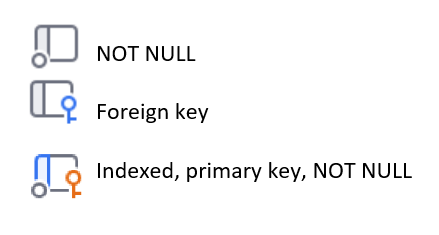
\includegraphics[scale=0.5]{figures/ERLegend}
    \caption{Legende: ER-Diagramm}
    \label{fig:er_diagramm_legend}
\end{figure}

\begin{figure}[ht]
    \centering
    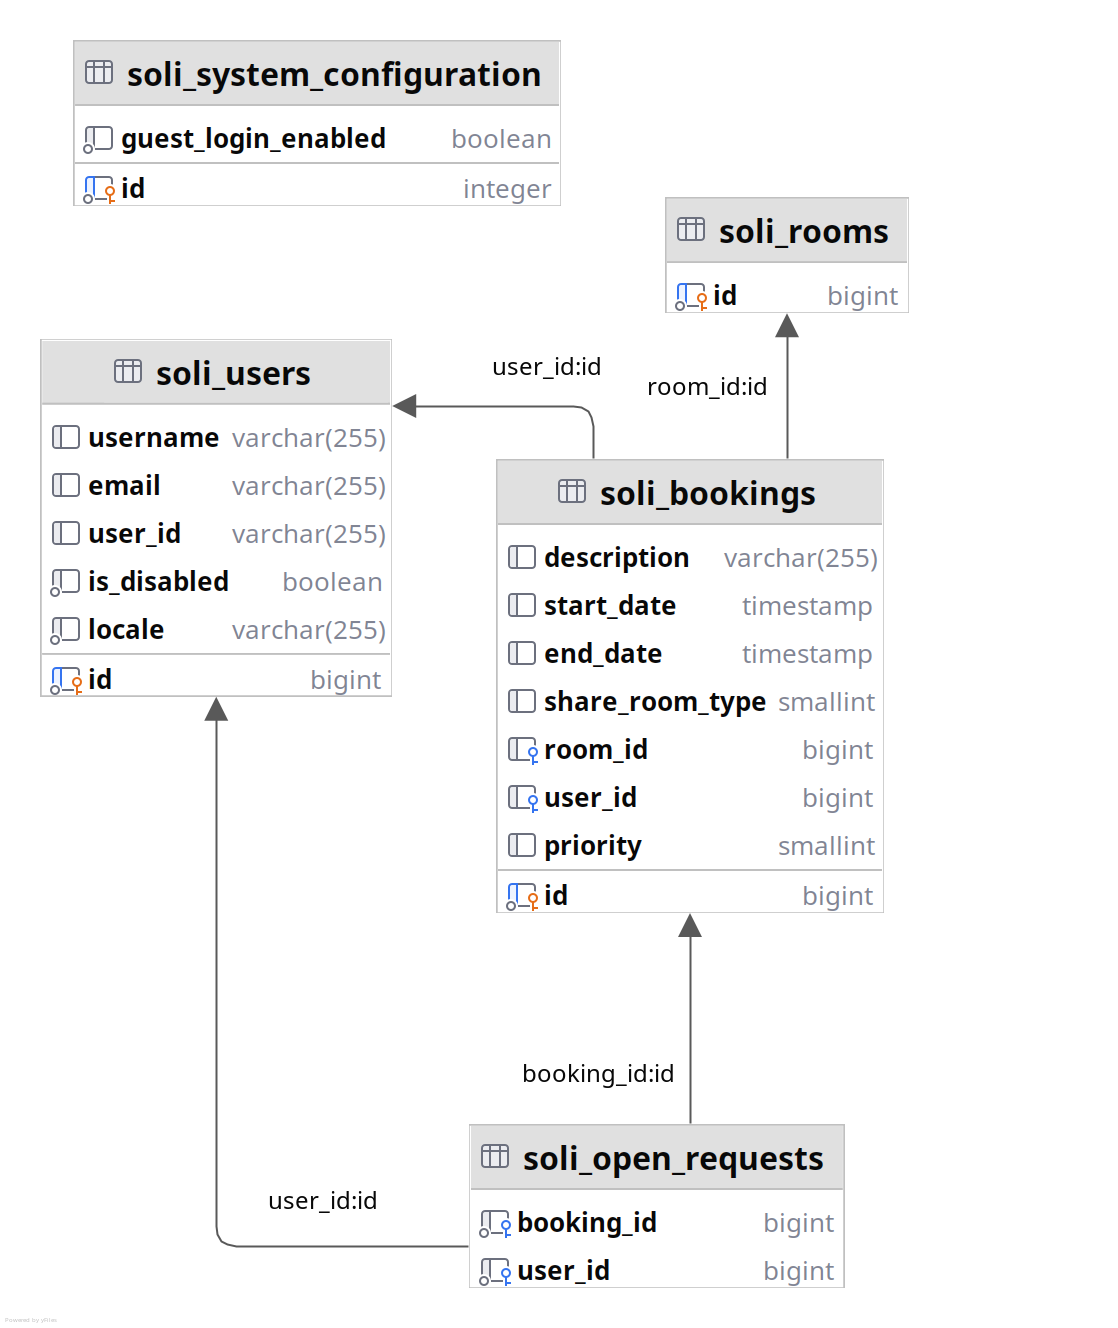
\includegraphics[width=\textwidth]{figures/database_old}
    \caption{ER-Diagramm}
    \label{fig:er_diagramm}
\end{figure}

\begin{figure}[ht]
    \centering
    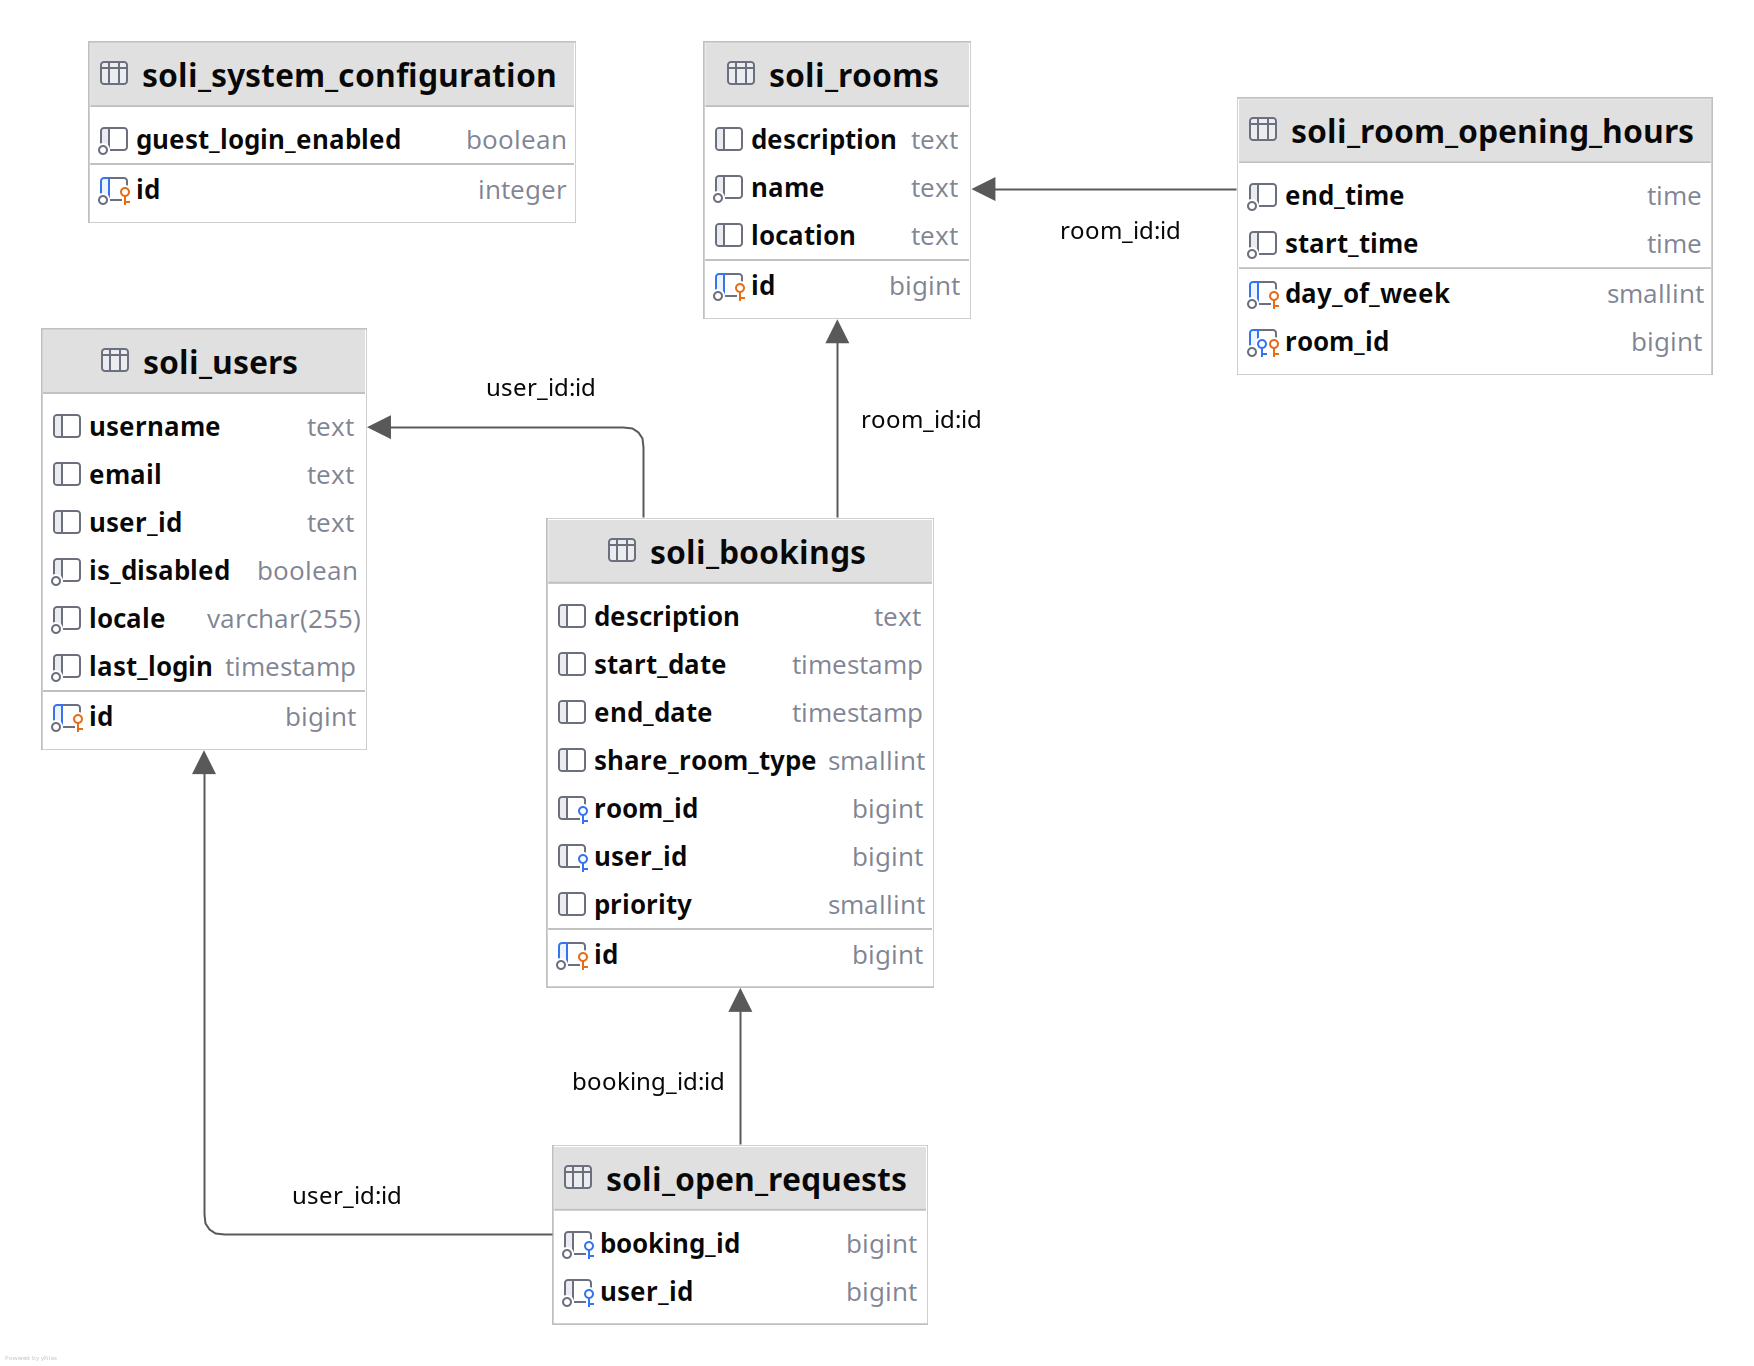
\includegraphics[width=\textwidth]{figures/database_new}
    \caption{Neues ER-Diagramm}
    \label{fig:er_diagramm_new}
\end{figure}
